\ifx\wholebook\relax \else

\documentclass[b5paper]{ctexart}
\usepackage[nomarginpar
  %, margin=.5in
]{geometry}

\addtolength{\oddsidemargin}{-0.05in}
\addtolength{\evensidemargin}{-0.05in}
\addtolength{\textwidth}{0.1in}

\usepackage[cn]{../prelude}

\setcounter{page}{1}

\begin{document}

\title{数的诞生}

\author{刘新宇
\thanks{{\bfseries 刘新宇} \newline
  Email: liuxinyu99@hotmail.com \newline}
  }

\maketitle
\fi

\markboth{数的诞生}{数的旅程}

\ifx\wholebook\relax
\chapter{数的诞生}
%% \numberwithin{Answer}{chapter}
%% \numberwithin{Exercise}{chapter}
\fi

\epigraph{一二三四五,金木水火土。\\
天地分上下,日月照今古。}{部编小学一年级\\
语文课本第一课}

数充满了我们的生活。例如报纸上这段新闻报道:“2024年巴黎奥运会(第33届奥运会)已于当地时间2024年8月1日闭幕。巴黎是继伦敦后的世界第2个至少3次举办夏奥会的城市。这是首届男女比例完全平衡的奥运会,男女运动员各为5250名。本届奥运会共设有32个大项,329个小项,共有206个国家和地区参赛,新增了滑板、冲浪、竞技攀岩和霹雳舞四个大项。中国代表团最终在巴黎奥运会上夺得40金27银24铜的优异成绩。”

这短短的180字中有14个数字。数是谁发明的?历史书上没有答案。数出现在所有历史文字记录中,数也许诞生在史前,伴随着语言和文字。要找到答案,我们有两条线索:1、追寻古老的历史物证,石刻、壁画、器物上关于数的印记;2、追溯数在语言演变中的痕迹。比如英文中的eleven (11)来自古英语endleofan,意思是(数到10还)剩余1;tweleve (12)来自twelf,意思是剩余2。

\section{罗塞塔石碑}
\index{罗塞塔石碑}

\begin{figure}[htbp]
 \centering
 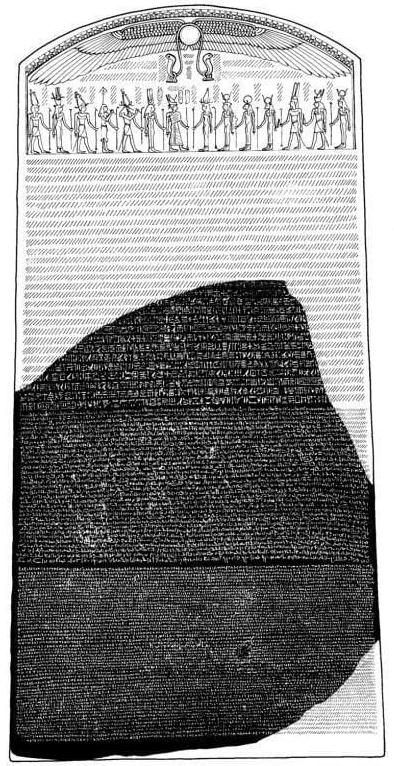
\includegraphics[scale=1.0]{img/Rosetta-stone-recons}
 \caption{古埃及罗赛塔石碑。石碑不完整,从中间断裂。}
 \label{fig:rosetta-stone-recons}
\end{figure}

走进大英博物馆第4展厅,有一件展品吸引着观众。这是一块残缺的石碑,长114厘米,宽72厘米,上面刻满了文字(\cref{fig:rosetta-stone-recons})。人们能一眼辨认出位于底部的内容是希腊字母(\cref{fig:rosetta-greek},参见\cref{ch:greek-letters}希腊字母表),但上面的部分犹如天书。仔细观察会发现余下的文字大致分成两种:一种是弯弯曲曲的符号,如\cref{fig:rosetta-demotic},位于石碑中部;另一种是奇妙的图案,如\cref{fig:rosetta-hieroglyphs},位于石碑上部。

\begin{figure}[htbp]
  \centering
  \subcaptionbox{古希腊文,共54行\label{fig:rosetta-greek}}{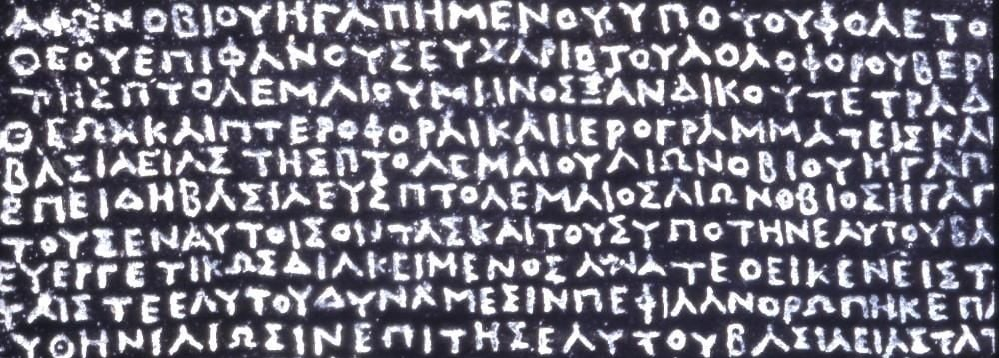
\includegraphics[scale=0.5]{img/Rosetta-Greek}} \\
  \subcaptionbox{古埃及世俗文字,是当时埃及平民使用的文字。共32行\label{fig:rosetta-demotic}}{\quad 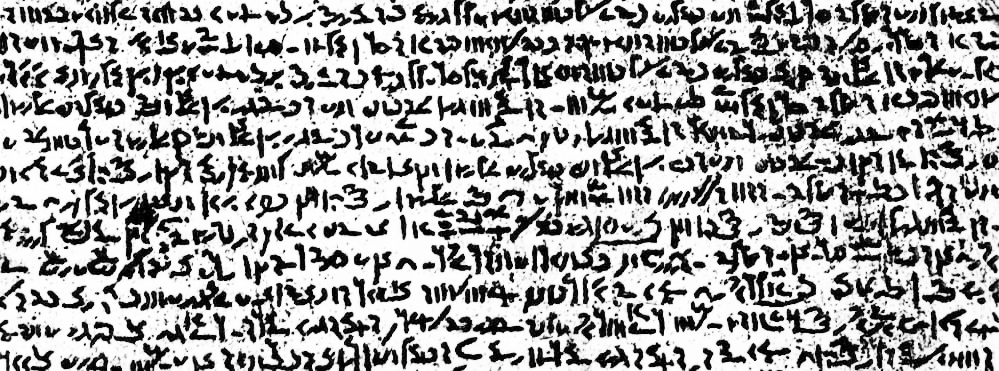
\includegraphics[scale=0.5]{img/Rosetta-Demotic}\quad} \\
  \subcaptionbox{古埃及象形文字,又称圣书体,代表献给神明的文字。共14行\label{fig:rosetta-hieroglyphs}}{\qquad 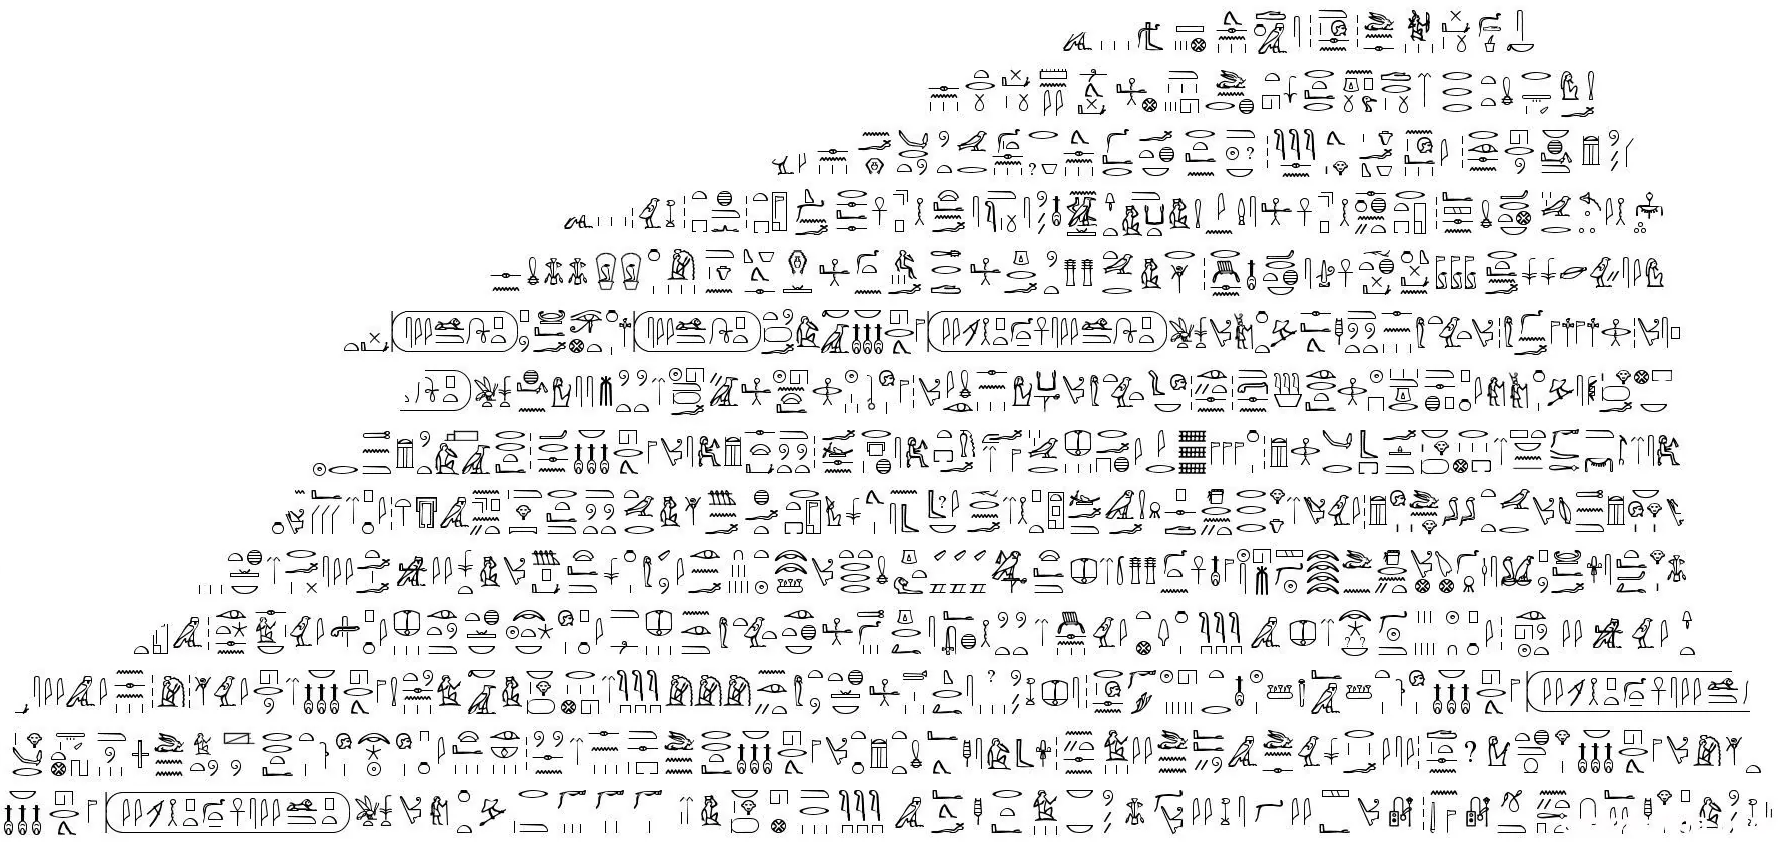
\includegraphics[scale=0.3]{img/Rosetta-Hieroglyphs-c}\qquad}
  \caption{罗赛塔石碑上的三种文字}
  \label{fig:rosetta-stone}
 \end{figure}

这一展品叫做罗塞塔石碑。1799年,拿破仑率领法军远征埃及。远征军有3万余人,各类舰只350艘,另有学者工程师146人。这位未来的法兰西皇帝从一名炮兵军官脱颖而出。他敏锐地看出数学不仅可以算出大炮的弹道,还关乎法兰西的国运。拿破仑的大军巧妙地避开了英国海军的封锁,7月2日攻占了埃及的亚历山大城,随即向开罗进军。7月15日,一位士兵在尼罗河三角洲前线的小镇罗塞塔(Rosetta)挖掘防御工事。他偶然发现了一块断碑砌在一段古老的墙中。尽管并不完整,这仍是一个重大的发现。法军指挥官决定把它送到拿破仑设立于开罗的埃及研究所,并于8月运抵开罗。根据发现地点,它被命名为罗塞塔石碑。1801年,英军击败了拿破仑,罗塞塔石碑也落入了英军之手。1802年2月,它被运抵英国朴次茅斯港,并最终收藏于大英博物馆。

这块石碑有何特殊之处呢?它上面用三种不同的文字记录了同一内容:公元前196年,13岁的国王托勒密5世加冕一周年。他从父亲托勒密4世袭得正统王位,并做了许多善行,如捐助神庙、减免税收等等。埃及当时处于托勒密王朝的统治之下,统治者是希腊人\footnote{马其顿国王亚历山大大帝征服了埃及。他死后,埃及总督托勒密一世于公元前305年自称国王建立王朝,统治埃及275年。}。国王宣称自己是法老。因此铭文使用了古埃及象形文字、古埃及世俗文字、希腊官方文字三种文字镌刻,并颁布全埃及各个神庙勒石立碑。而罗塞塔石碑就是其中之一,并且是至今唯一发现的一块。罗塞塔石碑于是成为了破解古埃及文字的钥匙。英国物理学家托马斯·杨\footnote{托马斯·杨(1773~1829),就是高中物理课本中杨氏双缝实验——发现光的干涉现象的物理学家。}和法国学者商博良通过研究此碑,成功破译了古埃及象形文字\cite{BM-RS-17}。

\section{古埃及和古巴比伦的计数系统}
\index{计数系统}

通过对古文字的破译,我们发现古埃及大约在公元前3400年就出现了表示数字的符号。是众多古文明中最早的(美索不达米亚大约在公元前3000年出现了数字符号,中国大约在公元前1600年出现了数字符号)。各文明中最早出现的数字符号是多是“|”、“||”、“||”或“-”、“=”、“$\equiv$”。这表明我们的老祖先是从“数数”开始认识数字的。很可能是采集、狩猎到更多的东西。随着生产生活的进步,人们逐渐认识更大的数,并逐渐从一数到了十——显然我们的祖先搬着手指头数数。但接下来遇到了困难。人只有两只手十个手指。这时有三种解决方法:(1)把脚也用上可以数到二十,但接下来会遇到同样的问题。(2)自由分组。在西伯利亚的尤卡吉尔语中有这样的例子:三和一、两个三、两个四、十差一等等。(3)固定分组。数到某一固定数目,例如十,分成一组,把这个组看成一个单位并起个名字。比如古埃及用$\cap$表示十。这样$\cap \cap$表示二十(古罗马用X表示十,I表示一。23表示为XXIII)。

\begin{figure}[htbp]
 \centering
 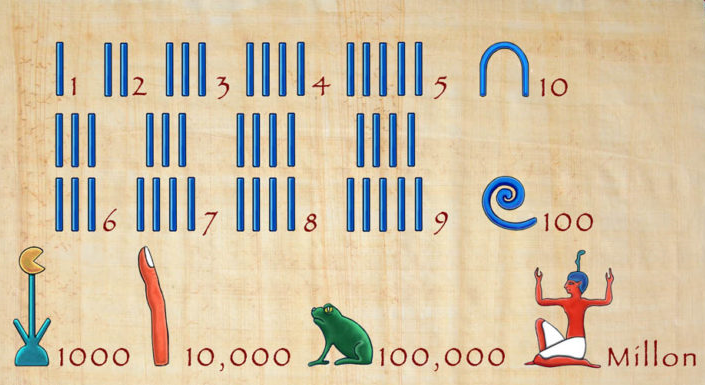
\includegraphics[scale=0.8]{img/hieroglyphic-numbers}
 \caption{古埃及象形文字中的数字符号。}
 \label{fig:egypt-hieroglyphic-numerals}
\end{figure}

为了建造宏伟的金字塔,古埃及人还创造了更大的单位符号,如\cref{fig:egypt-hieroglyphic-numerals}。他们用永恒之神(Heh)代表一百万,用蝌蚪表示十万,用弯曲的手指表示一万,莲花表示一千、弯曲的绳子表示一百……计数时按照单位分组,超出后就组成更大的单位。最后把每个单位的数目和单位表示的大小乘起来。\cref{fig:egypt-number-examples}给出了两个例子。

\begin{figure}[htbp]
 \centering
 \subcaptionbox{数字214427表示为$2(100000)+1(10000)+4(1000)+4(100)+2(10)+7(1)$}{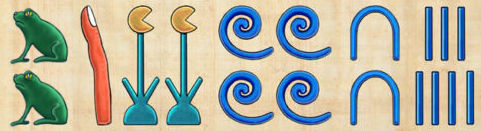
\includegraphics[scale=0.5]{img/egypt-num-eg2}}
 \subcaptionbox{古埃及埃德富(Edfu)神庙中的象形文字数字。表示1333330}{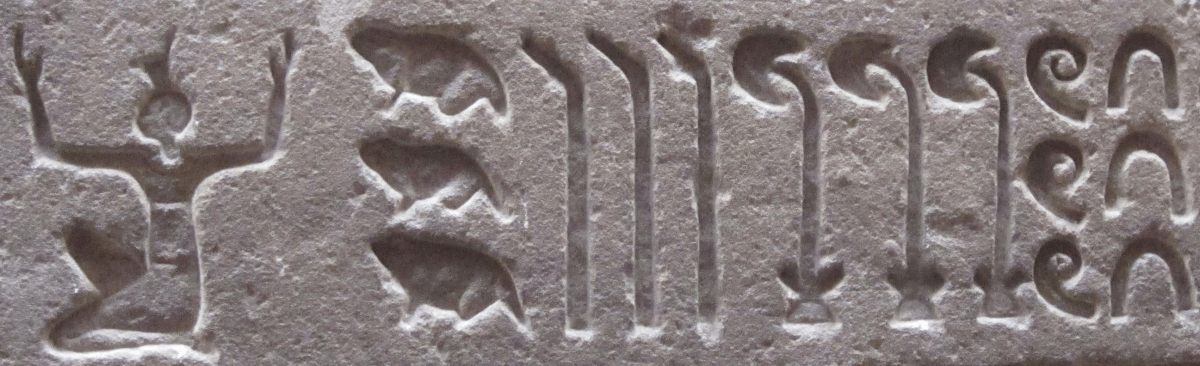
\includegraphics[scale=0.2]{img/Hieroglyphic-num-eg}}
 \caption{古埃及象形文字数字的例子}
 \label{fig:egypt-number-examples}
\end{figure}

尽管这种方法能够处理很大的数,但方法(2)自由分组对付小数字也很方便。古巴比伦人使用60进制(分组单位是60)。这种进制今天也出现在我们的日常生活中。60秒是1分,60分是1小时。所以1小时12分30秒,或写成1:12:30,包括$1(60\times 60) + 12(60) + 30 = 4350$秒。60对古巴比伦人足够大,所以他们在60以内使用自由分组法,超过60用$60^2$、$60^3$、$60^4$……分组。\cref{fig:babylonian-numerals}是古巴比伦楔形文字60以内的数字符号。古巴比伦人生活在美索不达比亚平原,在两河流域(位于底格里斯河、幼发拉底河之间的平原,现今的伊拉克境内)。他们在湿泥板上刻划文字,然后在阳光下晒干或用火烘干变硬。这些文字呈楔形。可以明显看出其中的规律:一是一个纵向的楔形,从一到九每数一就增加一个纵向的楔形。十变成了一个横向的楔形,从十一到十九是一个横向的楔形(10)加上相应纵向的楔形。二十是两个横向的楔形,然后重复这个规律。所以60以内的数字是横向的楔形个数乘以10加上纵向的楔形个数。

\begin{figure}[htbp]
 \centering
 \subcaptionbox{古巴比伦楔形文字中的数字符号\label{fig:babylonian-numerals}}{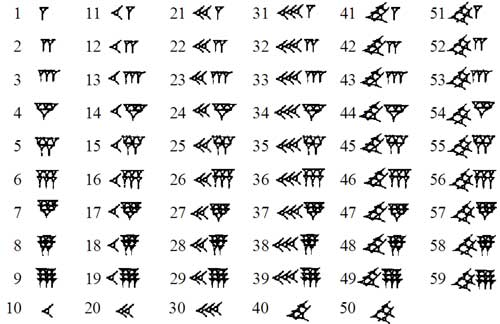
\includegraphics[scale=1.3]{img/Babylonian-numerals}} \\
 \subcaptionbox{古巴比伦楔形数字$1(60^3) + 19(60^2) + 21(60) + 54$\label{fig:babylonian-num-eg}}{
\includegraphics[scale=0.25]{img/Babylonian-num-eg}}
 \caption{古巴比伦数字}
\end{figure}

但60以上的数字展现出不一样的规律,如\cref{fig:babylonian-num-eg}所示。285714的60进制表示是1:19:21:54,但19写成了$20-1$。其中较小的纵向楔形表示减法,减数的上方有一个向右的楔形。可以看出,这并非是我们现代意义上严格的60进制,而是一种混合进制——60以内用十进制或减法表示。和古埃及相比,古巴比伦没有为$60$、$60^2$、$60^3$……创建单独的符号,而是依赖数字所在的位置决定单位的大小。最左边的数字表示有多少个1,向右的第二个位置上的数字表示有多少个60,第三个位置上的数字表示有多少个$60^2$,以此类推。这种方法叫做“位值制系统”。但由于缺乏0,古巴比伦的数字有歧义。直到约公元前300年后才偶尔出现了0,但只用于数字的中间而非结尾,无法区分出11和1100.古文字学者至今仍面临这个问题,只能通过上下文推测数值。

\section{古罗马和中国计数系统}
\index{乘法分组计数系统}

随着古罗马文明的崛起并建立起横跨欧亚非的帝国,罗马计数系统产生了巨大的影响,直到今天我们仍然可以在钟表盘上、建筑上、著作的章节编号上看到罗马数字(\cref{fig:clock-plate})。罗马数字的优点是只用少数几个符号,如I、V、X、C、M就够了。对于较小的数字很直观,例如III表示3,VII表示5 + 2 = 7,2025可表示为MMXXV(2个1000,2个10加5)。但是罗马数字的缺点是用法混乱。早期的罗马数字只包含加法,后来出现了“左减右加”的用法,如IV表示5 - 1 = 4,而VI表示5 + 1 = 6。这样IXX = (10 - 1) + 10 = 19,但19 = 10 + (10 - 1) = XIX就有歧义了:XIX还可以理解为(XI)X = 11 + 10 = 21。同样XVIII = 16,但16 = 8 + 8 = IIXXIIX和16 = (10 - 4) + 10 = IIIIXX都有歧义。其中IIIIXX出现在1388年巴黎的一份协定中来表示88\cite{LeVeque-Smith-25}。

\btab{|c|c|c|c|c|}
\hline
1 & 5 & 10 & 100 & 1000 \\
\hline
I & V & X  & C   & M \\
\hline
\etab

\begin{figure}[htbp]
 \centering
 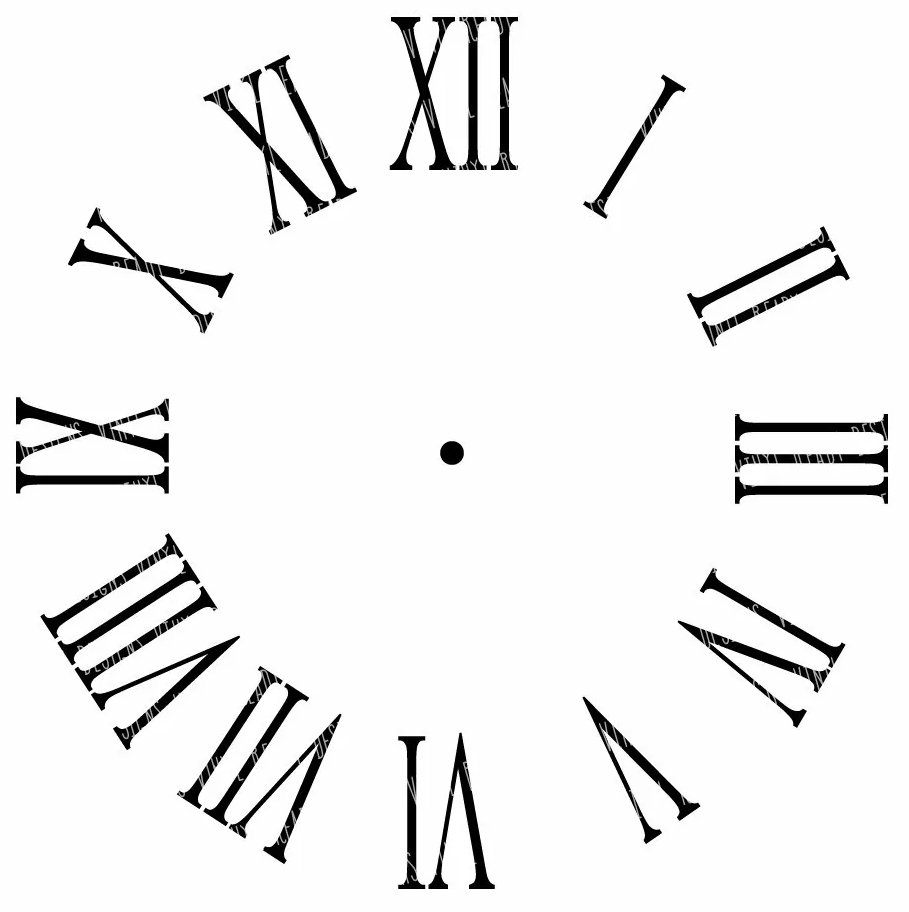
\includegraphics[scale=0.4]{img/clock-plate}
 \caption{钟表盘上的罗马数字}
 \label{fig:clock-plate}
\end{figure}

在古代中国产生了非常接近现代计数系统的十进制“乘法分组”法。华夏文明的前10个数字符号是:

\btab{cccccccccc}
一 & 二 & 三 & 四 & 五 & 六 & 七 & 八 & 九 & 十 \\
\etab

接下来中文没有出现英文中eleven(剩一)和twelve(剩二)的问题,而是直接进展到十一、十二……十九、二十……九十九。数字较小时,也使用廿(20)和卅(30),通常用在日历中。然后增加了百、千、万的分组单位。例如6147写为六千一百四十七,表示(六千)(一百)(四十)(七),即6个千、1个百、4个十、7个一,或6千1百4十7个,换成罗马单位相当于6M1C4X7I。每个数字$d_i$乘以单位的大小$u_i$,然后加到一起$d_nu_n + \cdots + d_1u_1$就是数值。这看起来和我们日常生活中熟悉的数字几乎一样了,可是几乎毕竟是几乎,究竟还差了一些。比如六千一百七,究竟是6170还是6107?汉字中不是有“零”么?可是在公元十世纪前的古代中国,零从来没有用在数学上。零是一个形声字,雨表形,令表声。本意是下雨。例如《诗经·豳风·东山》:我来自东,零雨其濛。引申意是落下,例如《诗经·郑风·野有蔓草》:野有蔓草,零露漙(tu\'{a}n)兮。《楚辞·离骚》:惟草木之零落兮,恐美人之迟暮。在可能成书于东汉时期的《九章算术》中,没有出现任何含有汉字零的数字。即使在宋元以后引入了零,但用法并不一致。例如103可以写成一百零三,也可以写成一百有三。《水浒传》里的好汉数目常读作一百单八将。在没有零的情况下,要想避免歧义就必须明确每个数字所代表的单位。这就需要给不同大小的分组单位命名或创造符号。随着数字的增大就需要更多的单位。但数的增加是无限的,而符号的数目是有限的,早晚有用光的时候。下表列出了中文和英文中越来越大的单位名称。

\begin{center}
% for Pinyin tones: \={a}, \'{a}, \v{}, \.{a}
\begin{tabular}{|l|r|l|r|l|r|}
\hline
百            & $100$      & 秭(z\v{i})    & $10^{24}$ &  \textbf{恒河沙}  & $10^{52}$ \\
\hline
千            & $1000$     & 穰(r\'{a}ng)  & $10^{28}$ & 阿僧祗(zh\={i})  & $10^{56}$ \\
\hline
万            & $10000$    & 沟            & $10^{32}$ & 那由他        & $10^{60}$  \\
\hline
亿            & $10^8$     & 涧            & $10^{36}$ &  不可思议      & $10^{64}$ \\
\hline
兆            & $10^{12}$  & 正            & $10^{40}$ &  无量大数      & $10^{68}$ \\
\hline
京            & $10^{16}$  & 载            & $10^{44}$ &               & \\
\hline
垓(g\={a}i)   & $10^{20}$  & 极            & $10^{48}$ &               & \\
\hline
\end{tabular}
\end{center}

可以看到,汉语中这些大单位词汇,有许多来自佛教。包括恒河沙,它表示1后面跟着52个0。英语中的大单位如下表。从一开始,每增加一千倍就有一个对应的单位。万进位和千进位的不同,也是文化上的一种差异。

\begin{center}
\begin{tabular}{|l|r|l|r|l|r|}
\hline
thousand & $10^{3}$ & quattuordecillion & $10^{45}$ & octovigintillion & $10^{87}$ \\
\hline
million & $10^{6}$ & quindecillion & $10^{48}$ & novemvigintillion & $10^{90}$ \\
\hline
billion & $10^{9}$ & sexdecillion & $10^{51}$ & trigintillion & $10^{93}$ \\
\hline
trillion  & $10^{12}$ & septdecillion & $10^{54}$ & untrigintillion & $10^{96}$ \\
\hline
quadrillion  & $10^{15}$ & octodecillion & $10^{57}$ & duotrigintillion & $10^{99}$ \\
\hline
quintillion  & $10^{18}$ & novemdecillion & $10^{60}$ & \textbf{googol} & $10^{100}$ \\
\hline
sexillion    & $10^{21}$ & vigintillion & $10^{63}$ & & \\
\hline
septillion   & $10^{24}$ & unvigintillion & $10^{66}$ & & \\
\hline
octillion    & $10^{27}$ & duovigintillion & $10^{69}$ & & \\
\hline
noniliion  & $10^{30}$ & trevigintillion & $10^{72}$ & & \\
\hline
decillion  & $10^{33}$ & quattuorvigintillion & $10^{75}$ & & \\
\hline
undecillion   & $10^{36}$ & quinvigintillion & $10^{78}$ & & \\
\hline
duodecillion  & $10^{39}$ & sexvigintillion & $10^{81}$ & & \\
\hline
tredecillion  & $10^{42}$ & seprvigintillion & $10^{84}$ & & \\
\hline
\end{tabular}
\end{center}

表中最后一个大单位古格尔(googol)是在1920年由9岁的米尔顿$\cdot$西洛塔(Milton Sirotta)想出的名字。这个数字是1后面跟着100个零。著名的互联网公司谷歌的名字就来自它。

\section{位值制计数系统}
\index{位值制计数系统}

在大航海时代,西班牙探险者在中美洲的尤卡坦半岛(位于墨西哥湾和加勒比海之间)发现玛雅文明创造出了完美的计数系统。\cref{fig:maya-numerals}给出了玛雅数字。类似古巴比伦的10-60混合进制,玛雅人使用5-20混合进制。20以内采用5进制,每数1点一个点,每数到5划一横线。20以上的数竖着写,并规范使用0做占位符,如\cref{fig:maya-numerals}。玛雅人的计数系统和玛雅历法相互影响。以地球围绕太阳旋转一周作为一个太阳年,每月20天。玛雅人很快发现$20 \times 18 = 360$,很接近一年。于是规定1年18个月,在加上5个禁忌日,一年恰好是365天。每4年再加上1天。这和我们现今太阳年的天数几乎一样。

\begin{figure}[htbp]
 \centering
 \subcaptionbox{20以内采用5进制}{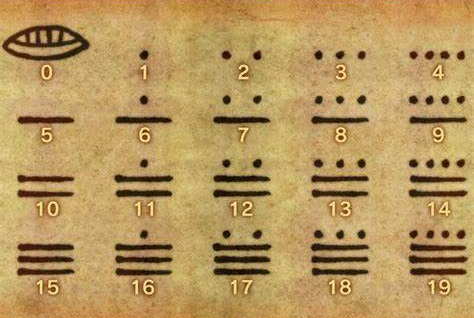
\includegraphics[scale=1.0]{img/Maya-numerals}} \qquad
 \subcaptionbox{$2(20^3) + 6(20) + 13 = 16133$}{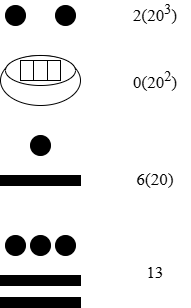
\includegraphics[scale=0.4]{img/Maya-num-eg}}
 \caption{玛雅数字}
 \label{fig:maya-numerals}
\end{figure}

无论是玛雅的20进制还是古巴比伦的60进制,都不需要额外命名单位,而是通过数字所在位置赋予大小的意义。这种方法叫做位值制计数系统(positional numeral system),归纳起来有3个要求:

\begin{enumerate}
\item 确定一个进制$b$\footnote{英文base的首字母}。如我们今天日常使用的$b = 10$、古巴比伦使用的$b = 60$、玛雅使用的$b = 20$。
\item 给1、2……$b-1$这些数字命名。例如汉语的一、二、三……九;英语的one, two, three, ..., nine;玛雅的点、点点……四点三划。
\item 代表0的符号。
\end{enumerate}

这样任何一个数$n$等于:

\be
n = a_m b^m + a_{m-1} b^{m-1} + \cdots + a_a b + a_0
\label{eq:pos-rep}
\ee

其中$a_i$是被命名的数字,包括0、1、2……$b-1$。$n$写为$a_ma_{m-1} \cdots a_0$。例如$2024 = 2 \times 10^3 + 0 \times 10^2 + 2 \times 10 + 4$, 其中$b = 10, m = 3, a_3 = 2, a_2 = 0, a_1 = 2, a_0 = 4$,恰好也写为2024。注意0在这里的起到了关键的“占位”作用——总共有2个千、2个十、4个一,但是没有百。0占据在百的位置上,这样其它数字才能“各就各位”,避免出现224这样的问题。我们再看一正一反两个例子:

\begin{example}
猫咪王国中,每只猫爪只有4个可动的指(\cref{fig:cat-paw}),左右共8个可动的指。如果采用8进制,并规定0的符号为“喵”,1到7为:(1)苗、(2)秒、(3)妙、(4)咪、(5)谜、(6)米、(7)蜜。王国一年的天数$365 = 5 \times 64 + 5 \times 8 + 5$,写成“谜谜谜”。$2024 = 5 \times 8^3 + 3 \times 8^2 + 7 \times 8 + 0$,写成“谜妙蜜喵”。

\begin{figure}[htbp]
 \centering
 
\includegraphics[scale=0.8]{img/cat-paw}
 \caption{猫爪}
 \label{fig:cat-paw}
\end{figure}

\end{example}

\begin{example}
\textbf{反例:}我国古代用天干地支纪年。天干有10个符号:甲、乙、丙、丁、戊、己、庚、辛、壬、癸;地支有12个符号:子、丑、寅、卯、辰、巳、午、未、申、酉、戌、亥。组合起来可以记录60以内的数字,从甲子开始,接下来天干地支各向前进一到已丑,然后是丙寅……到癸亥结束(\cref{fig:sexagenary})。比如2025年是农历乙巳年。乙的上一个天干符号是甲,巳的上一个地支符号是辰,所以前一年2024年是甲辰年,后一年2026年是丙午年。尽管我们不说“丙天午地”,看似用位置表示(第一个符号是天干、第二个符号是地支),但干支纪年\textbf{不是位值制计数法}。例如丙午并非一个甲子中的第$3 \times 10 + 7 = 37$年,而是第43年\footnote{除了查看\cref{fig:sexagenary}外,也可以这样计算:天干每10年循环,地支每12年循环。丙是天干中的第3个符号,午是地支中的第7个符号,所以丙午年除以10余3且除以12余7。60中除以10余3的数字有3、13……43、53,其中只有43除以12余7。}。

\begin{figure}[htbp]
 \centering
 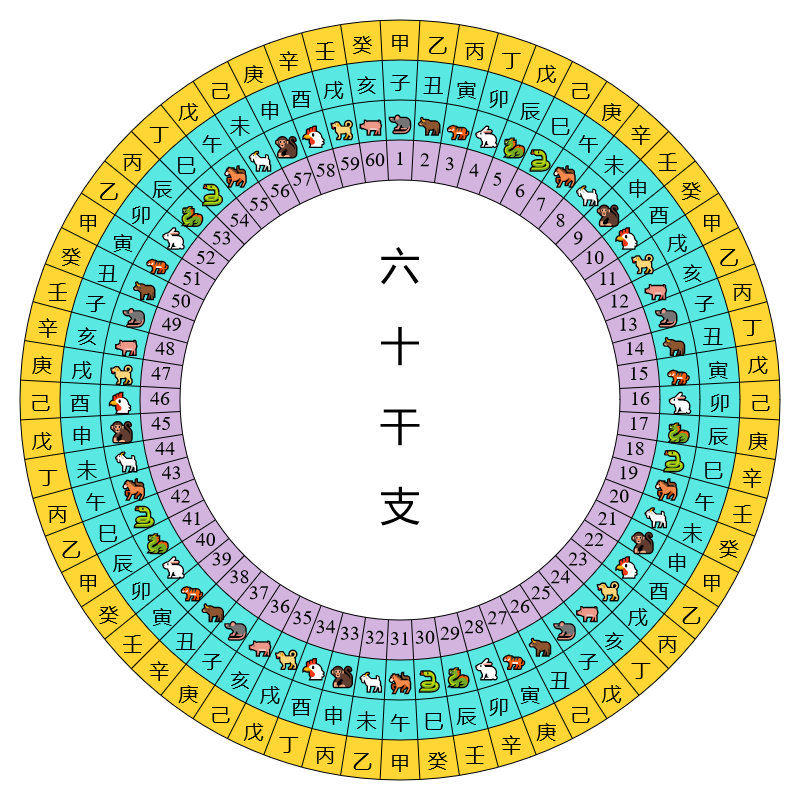
\includegraphics[scale=0.3]{img/sexagenary-chinese}
 \caption{干支纪年}
 \label{fig:sexagenary}
\end{figure}

\end{example}

罗马数字的一个问题就是歧义——一个数字有多种写法或一个写法可以代表不同的数字。位值制能解决这个问题么?明显8 = 08 = 008。我们在电梯、数字钟,汽车里程表上都见过类似的情况。可以在一个数字前放任意多个零而不改变值。如果对最高位的数字加以限制,规定\cref{eq:pos-rep}中的$a_m \neq 0$,那么一个数的位值制表示是唯一的(见\cref{qn:unique-pos-rep})。

% (1) Brahmi, 1st Century CE, (2) Indian (Gwalior), 9th Century, (3) Sanskrit Davanagari, Indian, 11th Cenntury, (4) West Arabic (Gubar? Gobar?), 11th Century, (5) East Arabic, 11th Centry, (still used in Turkey), (6) 15th Century, (7) 16th Century (Dürer)
\begin{figure}[htbp]
 \centering
 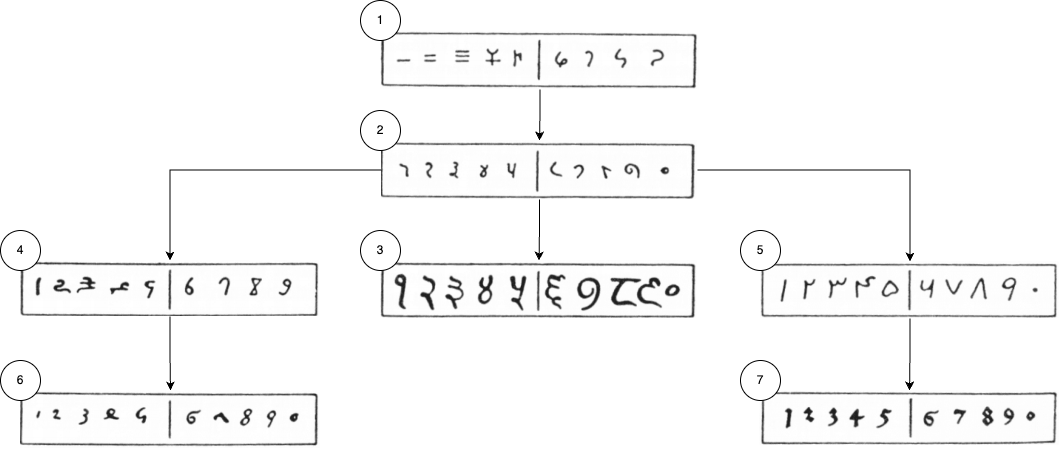
\includegraphics[scale=0.3]{img/Hindu-arabic-num}
 \caption{印度——阿拉伯数字的演进:1、婆罗门(Brahmi)数字出现在公元一世纪;2、印度瓜廖尔(Gwalior)数字包括0出现在公元九世纪;3、4、5、梵文天成体、东、西阿拉伯数字出现在公元十一世纪,其中西阿拉伯数字至今在土耳其仍然使用;6、7、十五世纪和十六世纪。}
 \label{fig:hindu-arabic-numerals}
\end{figure}

在历史的长河中,玛雅人和古巴比伦人的计数系统都湮没了。20和60以内的数字并非单一符号,混合进制难于计算。今天的现代位值制系统是印度文明发展出并经由阿拉伯人传入西方的,被称作“印度——阿拉伯系统”(Hindu-Arabic system)。在公元前三世纪,印度的碑铭中出现了1、4、6这样的符号;在公元一、二世纪的岩洞中,形如2、3、4、5、6、7、9的符号也出现了。可以看出2从二、3从三中演化的迹象,但直到公元九世纪以前,0仍未出现(\cref{fig:hindu-arabic-numerals})。印度人首先用一个点或小圆圈表示零,命名为sunya,梵文的意思是“空位”。传入阿拉伯后译为sifr,意思是“保持完整”。1140年,它伴随着阿拉伯学者花拉子密的著作被音译为拉丁文,最后变为今天英语中的zero。

\begin{mdframed}

\begin{center}
 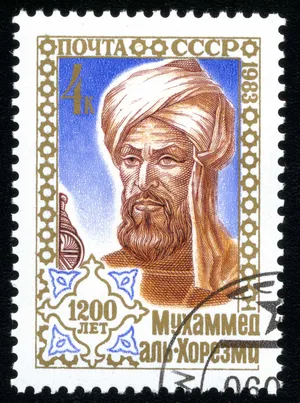
\includegraphics[scale=0.35]{img/Khwarizmi}
 \captionof{figure}{前苏联1983年发行的花拉子密纪念邮票}
 \label{fig:hindu-arabic-numerals}
\end{center}

公元七世纪初,阿拉伯文明崛起。罗马帝国分裂后,古希腊、拜占庭、印度的数学成果逐渐在八世纪汇集到阿拉伯帝国。阿拔斯王朝于公元830年在巴格达设立了著名的“智慧宫”,聚集了大批学者研究整理来自世界各地的天文地理资料和学术成果。公元813年,著名学者阿尔·花拉子密(al-Khwārizmī,约780~约850)来到巴格达,并成为智慧宫的主要学者之一。关于花拉子密的生平,我们知之甚少。甚至他的名字可能只是个“绰号”。阿拉伯文al是“来自”的意思,Khwārizmī是地名“花剌子模”,位于今天中亚的乌兹别克斯坦境内。金庸先生的小说《射雕英雄传》中有黄蓉帮着成吉思汗用计攻下花剌子模的故事,说的就是这个地方。花拉子密在数学方面完成了两部传世之作:《代数学》(成书于820年)和《印度数字算术》(成书于825年)。此外他还完成了地理和天文方面的著作。《代数学》的拉丁文译名为Hisab al-jabr w'al-muqabala,意思是还原与对消的科学。其中al-jabr后来演变为英文algebra。1859年清代学者李善兰与传教士伟烈亚力创造性地把它译为中文“代数”\cite{HanXueTao2009}。花拉子密在《代数学》中系统地给出了一元一次、二次方程的代数解法。但是他所在的时代还没有代数符号系统,因此完全使用文字来描述问题和解题步骤,并附加上几何解释来说明正确性。《印度数字算术》在十二世纪被翻译为拉丁文(Liber Algorismi de numero Indorum)并传入欧洲,促进了印度——阿拉伯十进制计数系统的传播。花拉子密名字的拉丁音译Algorismi后来成了“算法”一词Algorithm\cite{Britannica-25}。

%% https://www.britannica.com/print/article/317171
%% https://mathshistory.st-andrews.ac.uk/Biographies/Al-Khwarizmi/
\end{mdframed}

十进制位值制计数系统带来了巨大的优势。便于计算并可以处理任意大的数字。我们可以想象用罗马数字计算MMXXVV - CXXXVII有多么困难,而小学生也可以用竖式快速算出结果:

\begin{center}
\opsub[voperator=bottom]{2025}{137}
\end{center}

这仅仅是减法,更不用说乘除法了。尽管古代汉语中的计数系统并非位值制(见上一节),古代中国却发展出了一套严格意义上的位值制计算方法——筹算。筹算使用若干小棍进行计算。这些小棍用竹子制成叫做算筹\footnote{形声字“筹”的形旁是竹。也有用木头、兽骨、象牙、金属等材料的。}。它的发明是一个漫长的过程,但春秋战国时期已经普遍使用了。成语“运筹帷幄”、“一筹莫展”、“技高一筹”都反映了算筹的使用情况。算筹有横竖两种摆法,如\cref{fig:suanchou-digit}。如果个位竖着摆,则十位横着摆。这样交错摆放避免混淆。如果某一位是零,则空出不摆放\footnote{在计算过程中空位可能不明显造成混淆。后来人们在书写记录算筹运算结果时,就在应该是零的数位上写 “$\square$” 或 “〇”。}。算筹进行竖式计算非常方便,尤其是处理进位和借位。例如进位时只要把一个小棍摆到下一位就可以了。如\cref{fig:suanchou-eg}。

\begin{figure}[htbp]
 \centering
 \subcaptionbox{算筹数字的横竖摆法 \label{fig:suanchou-digit}}{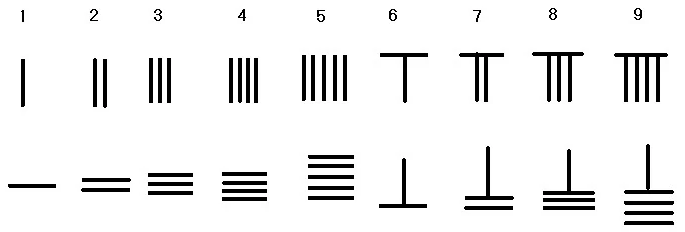
\includegraphics[scale=0.25]{img/suanchou-digit}}
 \subcaptionbox{算筹计算2025 - 137 \label{fig:suanchou-eg}}{\qquad
\includegraphics[scale=0.15]{img/suanchou-eg}\qquad}
 \caption{算筹}
\end{figure}

\index{斐波那契}
花拉子密的著作一开始只有少数学者了解。1202年斐波那契通过他的著作《算盘书》(Liber Abaci)进一步把印度——阿拉伯计数系统和计算方法介绍到欧洲。无独有偶,“斐波那契”其实也是个绰号。这位中世纪的数学家叫列奥纳多,来自比萨,所以称作比萨的列奥纳多。斐波那契来自拉丁文filius Bonacci,意思是波那契之子。斐波那契的父亲当时是商人,在北非以及地中海一带经商。斐波那契逐渐从埃及人、希腊人、西西里人、阿拉伯人那里学到个各种数字系统。他逐渐认识到了印度——阿拉伯计数系统的先进性。《算盘书》不仅包括位值制的记法,还讲解了如何计算利润率、记账、利息、汇率、度量衡换算、等实际问题。《算盘书》以其实用性大受欢迎,被广泛传抄。神圣罗马帝国皇帝腓特烈二世听说了斐波那契,在1220年邀请他到比萨。斐波那契接受了宫廷数学家的挑战,成功解决了所有题目,包括一道一元三次方程。他采用的数值解法给出了9位小数精度\cite{Gies-Carney-24}。今天,以他命名的“斐波那契数列”,即1、1、2、3、5、8……已经家喻户晓。我们将在第5章详细介绍这个有趣的数列。

\begin{figure}[htbp]
 \centering
 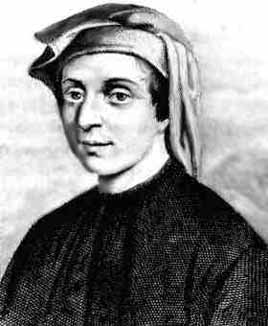
\includegraphics[scale=0.35]{img/Fibonacci}
 \caption{比萨的列奥纳多(斐波那契)1175-1250}
 \label{fig:Fibonacci}
\end{figure}

越来越多的学者和在各国往来贸易的商人们把印度——阿拉伯计数系统传播到了全球。它成了全人类的通用语言。十七世纪时,德国数学家莱布尼茨提出了二进制,它导致了二十世纪时计数系统再次产生了革命性的应用。电子计算机内部使用二进制对数字和信息编码。二进制只有0、1两种数字,尽管二进制表示很长,例如2025写成二进制是1111 1101 001,但0、1两种状态可以通过电路的通、断或电平(电压)的高、低方便地实现。还有一个好处:0、1可以对应逻辑的真、假;事物的有、无;答案的对、错,从而方便用机器统一处理数和逻辑,如\cref{tab:binary-arithmatic-logic}。

\begin{table}
\[\begin{array}{cccc}
  \begin{tabular}{c|c}
  $x$ & $1-x$ \\
  \hline
  0 & 1   \\
  \hline
  1 & 0   \\
  \end{tabular}
  &
  \begin{tabular}{c|c}
  $x$ & 非 $x$ \\
  \hline
  假 & 真  \\
  \hline
  真 & 假   \\
  \end{tabular}
   \quad & \quad
  \begin{tabular}{c|c|c}
  $x$ & $y$ & $x \times y$ \\
  \hline
  0 & 0 & 0  \\
  \hline
  0 & 1 & 0  \\
  \hline
  1 & 0 & 0  \\
  \hline
  1 & 1 & 1  \\
  \end{tabular}
  &
  \begin{tabular}{c|c|c}
  $x$ & $y$ & $x$ \text{与} $y$ \\
  \hline
  假 & 假 & 假 \\
  \hline
  假 & 真 & 假 \\
  \hline
  真 & 假 & 假 \\
  \hline
  真 & 真 & 真 \\
  \end{tabular}
\end{array}\]
\caption{二进制$1-x$与逻辑非的对应、乘法和逻辑与的对应}
\label{tab:binary-arithmatic-logic}
\end{table}

我们的祖先从狩猎、采集、计数开始,经过了四千余年才发展出了现代十进制位值制计数系统。数的诞生实在是一个漫长曲折的过程。它没有一个确定的发明者,而是在各个文明中独立产生于生产劳动,互相影响,逐渐发展,是人类群体性的进步。

\begin{Exercise}[label={ex:numerals}]
\Question{2025年深圳市南山区小学4年级期末数学考试中出现了这样一道题:计算$114 \times 21$,同学们用了不同的方法。在思路上这些方法有什么相同的地方?

\begin{multicols}{2}
\begin{enumerate}
  \renewcommand{\labelenumi}{\textcircled{\theenumi}}
  \item
    \begin{align*}
      114 \times 20 & = 2280 \\
      114 \times 1  & = 114 \\
      2280 + 114 & = 2394
    \end{align*}

  \item
    \begin{align*}
       & 114 \times 21 \\
     = & 114 \times 7 \times 3 \\
     = & 798 \times 3 \\
     = & 2394
    \end{align*}

  \item
    \[\begin{array}{cc}
    \begin{tabular}{|c|c|c|c|}
      \hline
      \times & 100  & 10  & 4 \\
      \hline
      20       & 2000 & 200 & 80 \\
      \hline
      1        & 100  & 10  & 4 \\
      \hline
    \end{tabular}  \quad
    \opadd[voperation=center,
           voperator=bottom]{2280}{114}
    \end{array}\]

  \item
    \opmul[displayshiftintermediary=all,
           voperator=bottom,
           voperation=top]{114}{21}
    \oplput(1,-2){$\cdots$ \opmul[style=text]{114}{1}}
    \oplput(1,-3){$\cdots$ \opmul[style=text]{114}{20}}
\end{enumerate}
\end{multicols}
这四个方法中,哪些利用了十进制位值制计数系统的优势?
}

\Question{可以利用$n = a_m b^m + a_{m-1} b^{m-1} + \cdots + a_a b + a_0$进行进制转换:
  \begin{enumerate}[(i)]
    \item 用$n$除以$b$得到余数$a_0$、商$q_0$。
    \item 把$n$替换为$q_0$,再次用$n$除以$b$得到余数$a_1$、商$q_1$。
    \item 把$n$替换为$q_1$,重复上述步骤知道商$q_m = 0$。
  \end{enumerate}
  则$n$的$b$进制表示为$a_m \cdots a_1a_0$。请将十进制数123转换为(a)玛雅文;(b)古巴比伦文;(c)计算机二进制表示。
}

\Question{如果你会编程,请用自己熟悉的语言实现二进制到十进制的相互转换。}

\Question{证明一个数的位值制表示是唯一的。提示:考虑如果一个数有两种表示会怎样? \label{qn:unique-pos-rep}}
\end{Exercise}

\begin{Answer}[ref={ex:numerals}]
\Question{ \textcircled{1}、\textcircled{3}、\textcircled{4} }

\Question{将十进制数123转换为(a)玛雅文;(b)古巴比伦文;(c)计算机二进制表示。
}

\Question{编程实现二进制到十进制的相互转换。}

\Question{证明一个数的位值制表示是唯一的。

\begin{proof}
假设一个数还有另一个表示。如果它们的位数不同,我们在较短的前面添加0,使它们一样长。令补0后的表示分别为$a_{m} a_{m-1} \cdots a_1 a_0$和$c_m c_{m-1} \cdots c_1 c_0$。按照\cref{eq:pos-rep}计算的值相等,即:
\[
  a_m b^m + a_{m-1} b^{m-1} + \cdots + a_1 b + a_0 = c_m b^m + c_{m-1} b^{m-1} + \cdots + c_1 b + c_0
\]

将$a_0$和$c_0$移到右边,剩下的移到左边:

\[
  (a_m - c_m) b^m + (a_{m-1} - c_{m-1}) b^{m-1} + \cdots + (a_1 - c_1) b = c_0 - a_0
\]

左边可以被$b$整除,所以$c_0 - a_0$也可以被$b$整除。由于$c_0$、$a_0$都只能是0到$b - 1$的整数,所以它们的差只能是$1 - b, \dots , -1, 0, 1, \dots b - 1$中的一个。但其中只有0能被$b$整除。所以$c_0 - a_0 = 0$,即$c_0 = a_0$。

接下来$(a_m - c_m) b^m + (a_{m-1} - c_{m-1}) b^{m-1} + \cdots + (a_1 - c_1) b = 0$。由于$b \neq 0$,两边除以$b$,然后将$a_1$和$c_1$移动到左边:

\[
  (a_m - c_m) b^m + (a_{m-1} - c_{m-1}) b^{m-1} + \cdots + (a_2 - c_2) b = c_1 - a_1
\]

同样可以推出$c_1 = a_1$。重复这个步骤$m$次,最后得到$a_m = c_m$。这就证明了两种表示是一样的,即位值制表示是唯一的。
\end{proof}
}
\end{Answer}


\ifx\wholebook\relax \else
\section{参考答案}
\shipoutAnswer

\begin{thebibliography}{99}

\bibitem{BM-RS-17}
British Museum. ``Everything you ever wanted to know about the Rosetta Stone''. British Museum blog, 14 July. 2017, \url{https://www.britishmuseum.org/blog/everything-you-ever-wanted-know-about-rosetta-stone}. Accessed 14 February 2025.

\bibitem{LeVeque-Smith-25}
LeVeque, William Judson, Smith, David Eugene. ``numerals and numeral systems''. Encyclopedia Britannica, 7 Jan. 2025, \url{https://www.britannica.com/science/numeral}. Accessed 14 February 2025.

\bibitem{HanXueTao2009}
韩雪涛. 好的数学——“下金蛋”的数学问题 [M]. 长沙:湖南科学技术出版社, 2009. %ISBN: 9787535756725

\bibitem{Britannica-25}
The Editors of Encyclopaedia Britannica. "al-Khwārizmī". Encyclopedia Britannica, 13 Feb. 2025, \url{https://www.britannica.com/biography/al-Khwarizmi}. Accessed 18 February 2025.

\bibitem{Gies-Carney-24}
Gies, Frances Carney. "Fibonacci". Encyclopedia Britannica, 2 Dec. 2024, https://www.britannica.com/biography/Fibonacci. Accessed 18 February 2025.

%% \bibitem{wiki-number}
%% Wikipedia. ``古代计数系统的历史''. \url{https://en.wikipedia.org/wiki/History_of_ancient_numeral_systems}

%% \bibitem{trip-to-number-kingdom}
%% [美]\ 卡尔文$\cdot$C$\cdot$克劳森\ 著\ 袁向东、袁钧\ 译. ``数学旅行家:漫游数王国''. 上海教育出版社。ISBN: 7-5320-7883-3/G $\cdot$ 7972

%% \bibitem{wiki-babylonian-num}
%% Wikipedia. ``古巴比伦数字''. \url{https://en.wikipedia.org/wiki/Babylonian_numerals}

\end{thebibliography}

\expandafter\enddocument
%\end{document}

\fi
